\section{Counting Problems}

\subsection{Stirling numbers of the first kind} These are the number of permutations of $[n]$ with exactly $k$ disjoint cycles. They obey the recurrence:

  \begin{equation*}
    \stirlingfirst{n}{k} = (n-1)\stirlingfirst{n-1}{k} + \stirlingfirst{n-1}{k-1},
  \end{equation*}
  
  \begin{equation*}
    \stirlingfirst{0}{0} = 1, \stirlingfirst{n}{0} = \stirlingfirst{0}{n} = 0
  \end{equation*}
  
\begin{itemize}
    \item The sum products of the $\binom{n}{k}$ subsets of size $k$ of $\{0, 1, \dots, n-1\}$ is $\stirlingfirst{n}{n-k}$.
    
    \item $\sum_{k=0}^n \stirlingfirst{n}{k} = n!$

    \item $\sum_{k=0}^{n}\stirlingfirst{n}{k}x^k = x(x-1)(x-2)...(x-n+1)$
\end{itemize}

\subsection{Stirling numbers of the second kind} These are the number of ways to partition $[n]$ into exactly $k$ non-empty sets. They obey the recurrence:
  \begin{equation*}
    \stirlingsecond{n}{k} = k\stirlingsecond{n-1}{k} + \stirlingsecond{n-1}{k-1}
  \end{equation*}
  
  \begin{equation*}
    \stirlingsecond{0}{0} = 1, \stirlingsecond{n}{0} = \stirlingsecond{0}{n} = 0
  \end{equation*}

  A ``closed'' formula for it is:
  \begin{equation*}
    \stirlingsecond{n}{k} = \frac{1}{k!}\sum_{j=0}^k (-1)^{k-j} \binom{k}{j} j^n
  \end{equation*}

\newcommand{\eulerian}[2]{\genfrac{\langle}{\rangle}{0pt}{}{#1}{#2}}
\subsection{Eulerian numbers} 
Eulerian numbers $\eulerian{n}{k}$ count the number of permutations of $[n]$ with exactly $k$ ascents (positions $i$ such that $p_i < p_{i + 1}$). They satisfy the recurrence:
\begin{equation*}
    \eulerian{n}{k} = (k+1)\eulerian{n-1}{k} + (n-k)\eulerian{n-1}{k-1}
\end{equation*}

\begin{equation*}
    \eulerian{0}{0} = 1, \quad \eulerian{n}{0} = \eulerian{n}{n-1} = 1
\end{equation*}

A ``closed'' formula for Eulerian numbers is given by:
\begin{equation*}
    \eulerian{n}{k} = \sum_{j=0}^{k+1} (-1)^j \binom{n+1}{j} (k+1-j)^n
\end{equation*}

\subsection{How many functions \texorpdfstring{$f \colon [n] \rightarrow [k]$}{} are there?} 

%\stirlingsecond{n}{k}
$$
\begin{array}{|c|c||c|c|c|}
    \hline
    \cellcolor{gray!40} [n] & \cellcolor{gray!40} [k] & \cellcolor{gray!40} \text{Any } f & \cellcolor{gray!40} \text{Injective} & \cellcolor{gray!40} \text{Surjective}
    \\ \hline \hline \text{dist} & \text{dist} & k^n & \frac{k!}{(n-k)!} & k!\stirlingsecond{n}{k}
    \\ \hline \text{indist} & \text{dist} & \binom{k+n-1}{n} & \binom{k}{n} & \binom{n-1}{n-k}
    \\ \hline \text{dist} & \text{indist} & \sum_{i = 1}^k \stirlingsecond{n}{i} & [n \le k] & \stirlingsecond{n}{k}
    \\ \hline \text{indist} & \text{indist} & \sum_{i = 1}^k p_i(n) & [n \le k] & p_k(n)\\
    \hline
\end{array}
$$

Where $p_k(n)$ is the number of ways to partition $n$ into $k$ terms.

    
\subsection{Derangement} A derangement is a permutation that has no fixed points. Let $d_n$ be the number of ways of derangement of a sequence of the sequence $1\dots n$. We have the recurrence $d_n=(n-1)(d_{n-1}+d_{n-2})$. Moreover, $d_n$ is the closest integer to $\frac{n!}{e}$.

$$d_n = n!\sum_{i=0}^{n}\frac{(-1)^i}{i!}$$

\subsection{Bell numbers} These count the number of ways to partition $[n]$ into subsets. They obey the recurrence:

\begin{equation*}
    \mathcal{B}_{n+1} = \sum_{k=0}^n \binom{n}{k} \mathcal{B}_k
\end{equation*}

\bigskip
\
\begin{tabular}{|c|c|c|c|c|c|c|c|c|}
\hline
\cellcolor{gray!40} x&5&6&7&8&9&10&11&12 \\ \hline
\cellcolor{gray!40} $\mathcal{B}_x$&52&203&877&4.140&21.147&115.975&678.570&4.213.597 \\ \hline
\end{tabular}
\

\subsection{Bernoulli numbers}

The Bernoulli numbers $B_m$ satisfy the recursive relation:

$$
B_m = 1 - \sum_{k=0}^{m - 1} \binom{m}{k} \frac{B_k}{m-k+1}, \quad \text{for } m \geq 1, \text{ with } B_0 = 1.
$$

\subsubsection*{Faulhaber's Formula}

These numbers can be used to compute the sum of powers of integers:

$$
\sum_{k=1}^{n} k^m = \frac{1}{m+1} \sum_{k=0}^{m} \binom{m+1}{k} B_k n^{m+1-k}.
$$

% \subsection{Eulerian numbers} 
% The Eulerian number $T(n,k)$ is the number of permutations of the numbers from $1$ to $n$ in which exactly $k$ elements are greater than the previous element (permutations with $k$ ``ascents'').
% 
% %http://oeis.org/A179457
% 
% $$ T(n,k) = \sum_{j = 0}^k (-1)^j (k-j)^{(n+1)} \binom{n+1}{j}$$


\subsection{Burside's Lemma}
    Let $G$ be a group that acts on a set $X$. The Burnside Lemma states that the number of distinct orbits is equal to the average number of points fixed by an element of G.
    $$T = \frac{1}{|G|} \sum_{g \in G} |\texttt{fix}(g)|$$
    Where a orbit $\texttt{orb}(x)$ is defined as
    $$\texttt{orb}(x) = \{y \in X : \exists g \in G \ gx = y \}$$
    and $\texttt{fix}(g)$ is the set of elements in $X$ fixed by $g$
    $$\texttt{fix}(g) = \{x \in X : gx = x\}$$
    
    \textbf{Example:} With $k$ distinct types of beads how many distinct necklaces of size $n$ can be made? Considering that two necklaces are equal if the rotation of one gives the other.
    \begin{center}
    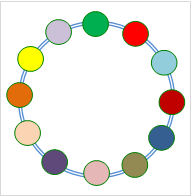
\includegraphics[scale=.6, keepaspectratio]{img/Burnside.png}
    \end{center}
    $$T = \frac{1}{n+1} \sum_{i=0}^{n}k^{gcd(i, n)}$$
    
\subsection{Catalan Numbers}

1, 1, 2, 5, 14, 42, 132, 429, 1430, 4862, 16796, 58786, 208012, 742900, 2674440, 9694845, 35357670, 129644790, 477638700, 1767263190, 6564120420, 24466267020, 91482563640, 343059613650, 1289904147324, 4861946401452, 18367353072152, 69533550916004, 263747951750360, 1002242216651368.\\

$$C_n = \frac{1}{n+1}\binom{2n}{n} = \frac{(2n)!}{(n+1)!n!} = \prod_{k=2}^{n} \frac{n+k}{k}, \quad n \geq 0$$\\


Applications:
\begin{itemize}

\item $C_n$ counts the number of expressions containing n pairs of parentheses which are correctly matched.
    $$((()))  \qquad  ()(())  \qquad  ()()()  \qquad  (())()  \qquad  \dots $$


\item Successive applications of a binary operator can be represented in terms of a full binary tree. (A rooted binary tree is full if every vertex has either two children or no children.) It follows that $C_n$ is the number of full binary trees with n + 1 leaves:\\
\begin{center}
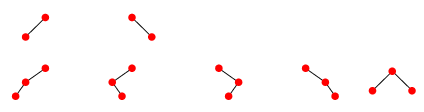
\includegraphics[scale=0.5]{img/catalan_tree.png}
\end{center}

\item $C_n$ is the number of different ways a convex polygon with n + 2 sides can be cut into triangles by connecting vertices with straight lines (a form of Polygon triangulation). The following hexagons illustrate the case n = 4:

\begin{center}
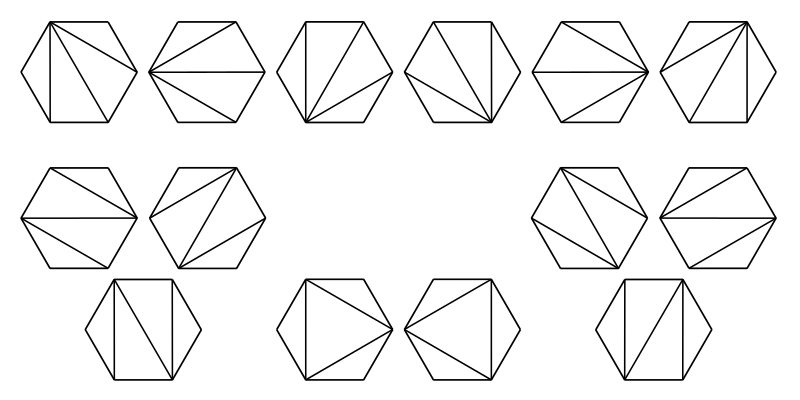
\includegraphics[scale=0.30]{Catalan-Hexagons-example.png}
\end{center}

\item There is also the recursive formula $C_n = \displaystyle\sum_{i=0}^{n - 1} C_i C_{n - 1 - i}$, which can be useful in some problems. More generally,

$$
\displaystyle\sum_{a_0+a_1+...+a_{k} = n}{C_{a_0} C_{a_1} ... C_{a_{k}}} = \displaystyle\frac{k+1}{n+k+1}\displaystyle{2n+k \choose n}
$$

\end{itemize}

\subsection{Central Binomial Coefficient}

To number of of subsets $T$ of $S = \{ \underbrace{1, 1, \dots, 1}_{n}, \underbrace{-1, -1, \dots, -1}_{n} \}$ that sum to 0 is

$$ \sum_{k=0}^n \binom{n}{k}^2 = \binom{2n}{n} = \frac{2n!}{\left(n!\right)^2} \approx \frac{2^{2n}}{\sqrt{n \cdot \pi}} $$

\begin{itemize}
    \item  The number of factors of 2 in $\binom{2n}{n}$ is equal to the number of 1's in the binary representation if $n$.
    
    \item $\binom{2n}{n}$ is never squarefree for $n > 4$.
\end{itemize}

